\chapter{Innover}
\label{cp:innover}

La phase \textit{Innover} de la démarche DMAIC vise à concevoir des solutions nouvelles permettant de supprimer les causes racines des non-conformités identifiées lors des phases précédentes. Dans ce projet, l'innovation porte sur l'intégration d'un modèle d'apprentissage automatique pour détecter automatiquement les \textit{silver faces} $\bullet$ des surfaces dégénérées difficiles à identifier par une règle déterministe simple.

Ce chapitre présente l'approche complète : extraction des caractéristiques géométriques, construction du modèle de régression logistique, analyse des performances et recommandations pour la mise en production dans un pipeline CATIA~V5.

% ============================================================
\section{Détection des \textit{Silver Faces} par Régression Logistique}
\label{sec:innover-silver-faces}
% ============================================================

\subsection{Problématique}
\label{subsec:problematique}

La macro existante est entièrement \textbf{basée sur des règles} et utilise exactement \textbf{une seule caractéristique} pour prendre chaque décision~:

\begin{equation}
    \text{Aire}\;(\text{mm}^2) < 0{,}01 \;\Rightarrow\; \textit{silver face}
    \label{eq:decision-rule-old}
\end{equation}

Cette approche est fragile. Les deux constantes arbitraires $\bullet$ \texttt{SEUIL\_MM2~=~0.01} et \texttt{SEUIL\_DELETE~=~0.0001} $\bullet$ ont été fixées manuellement par un ingénieur. Elles ne peuvent pas s'adapter~:

\begin{itemize}
    \item \textbf{Aux domaines industriels différents} $\bullet$ les tolérances aérospatiales et automobiles diffèrent d'ordres de grandeur.
    \item \textbf{Aux styles de modélisation différents} $\bullet$ les pièces importées en IGES et les pièces modélisées nativement dans CATIA présentent des propriétés géométriques très différentes.
    \item \textbf{Au contexte} $\bullet$ une surface de $0{,}008~\text{mm}^2$ adjacente à une aube de turbine constitue un \textit{défaut critique}~; la même aire sur un panneau décoratif n'est que du \textit{bruit}.
\end{itemize}

L'apprentissage automatique remplace ces seuils figés par une \textbf{fonction de décision apprise} à partir de l'historique réel des corrections.

% ============================================================
\subsection{Caractéristiques géométriques utilisées}
\label{subsec:features}
% ============================================================

Quatre indicateurs géométriques sont extraits pour chaque surface afin de capturer sa forme de manière discriminante.

La \textbf{compacité} (ou quotient isopérimétrique) est la métrique la plus puissante. Elle mesure l'écart entre la forme d'une surface et un cercle parfait~:

\begin{equation}
    C = \frac{4\pi A}{P^2}, \qquad C \in (0,\,1]
    \label{eq:compacite}
\end{equation}

où $A$ désigne l'aire et $P$ le périmètre de la surface. Un cercle parfait donne $C = 1$~; une forme extrêmement allongée ou irrégulière tend vers $C \approx 0$. Le \textbf{rapport d'aspect} complète cette information en mesurant l'élongation directe de la boîte englobante~:

\begin{equation}
    AR = \frac{L_{\max}}{L_{\min}}
    \label{eq:aspect-ratio}
\end{equation}

où $L_{\max}$ et $L_{\min}$ désignent respectivement la plus grande et la plus petite dimension. Un carré donne $AR = 1$~; une \textit{silver face} typique présente $AR \gg 60$. Enfin, l'\textbf{aire} $A$ (en mm²) et le \textbf{périmètre} $P$ (en mm) fournissent une information brute sur la taille absolue de la surface.

La \autoref{fig:distribution} illustre la distribution de ces quatre caractéristiques sur l'ensemble des~1\,500 surfaces du jeu de données.

\begin{figure}[H]
    \centering
    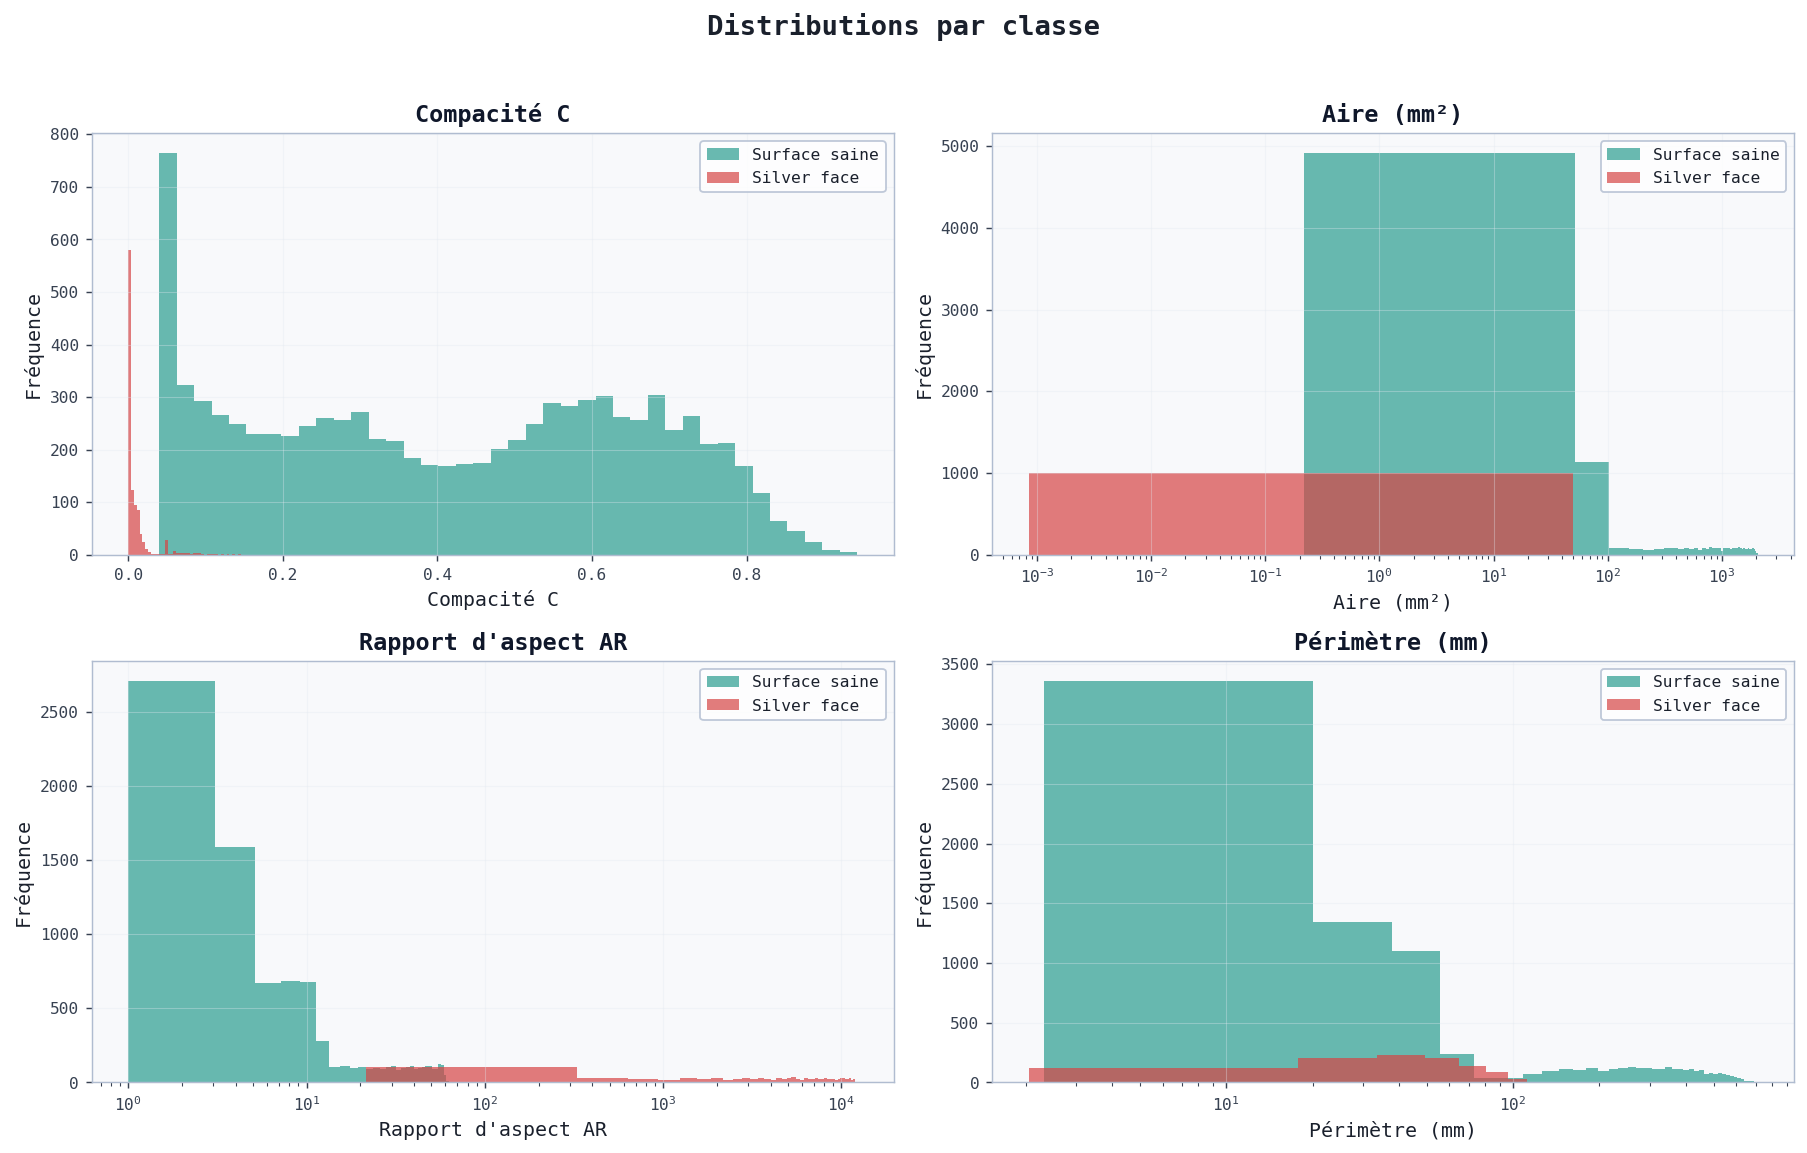
\includegraphics[width=\textwidth]{image/AI-SILVER-FACE/fig1_distribution.png}
    \caption{Distributions des quatre caractéristiques par classe (vert~: surface saine, rouge~: \textit{silver face}).}
    \label{fig:distribution}
\end{figure}

L'analyse de ces distributions révèle que la \textbf{compacité} et le \textbf{rapport d'aspect} sont les caractéristiques les plus discriminantes au premier degré~: les deux classes présentent des distributions quasi disjointes pour ces deux indicateurs. À l'inverse, l'aire et le périmètre offrent une séparation partielle mais insuffisante à eux seuls $\bullet$ ils jouent un rôle d'affinage dans les cas ambigus.

% ============================================================
\subsection{Espace des caractéristiques}
\label{subsec:feature-space}
% ============================================================

La \autoref{fig:feature-space} représente la distribution des 1\,500 surfaces dans l'espace des caractéristiques. Les surfaces saines apparaissent en vert, les \textit{silver faces} en rouge.

\begin{figure}[H]
    \centering
    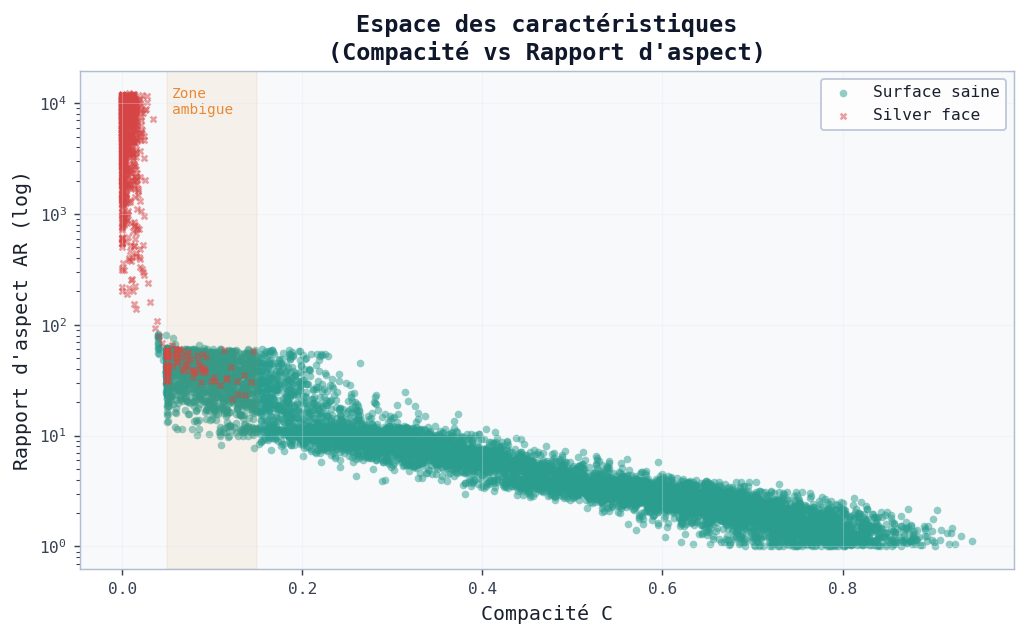
\includegraphics[width=0.9\textwidth]{image/AI-SILVER-FACE/fig2_feature_space.png}
    \caption{Compacité $C$ vs rapport d'aspect $AR$ : cluster \textit{silver face} (rouge) à faible $C$ et $AR$ élevé ; zone ambiguë en beige.}
    \label{fig:feature-space}
\end{figure}

Dans le plan Compacité $\times$ Rapport d'aspect, les deux classes se séparent nettement~: les \textit{silver faces} occupent la région de faible compacité ($C < 0{,}15$) et de rapport d'aspect élevé ($AR > 60$), tandis que les surfaces saines se concentrent dans la région de forte compacité ($C > 0{,}5$) et de faible rapport d'aspect ($AR < 20$). La zone d'ambiguïté, encadrée en beige, correspond à $C \in [0{,}05,\, 0{,}15]$ et $AR \in [30,\, 60]$~: des surfaces saines très allongées peuvent y coexister avec des \textit{silver faces} modérées.

Cette visualisation confirme le rôle central de la compacité $C$ et du rapport d'aspect $AR$ comme caractéristiques principales du modèle~: leur pouvoir discriminant est maximal, et leur combinaison permet de délimiter une frontière de décision claire et robuste. Le modèle de régression logistique exploite précisément cette structure géométrique pour séparer les deux classes avec un minimum de mauvaises classifications.

% ============================================================
\section{Modèle : Régression Logistique}
\label{sec:modele-rl}
% ============================================================

\subsection{Normalisation des données}
\label{subsec:normalisation}

Avant l'entraînement, chaque caractéristique est normalisée par le \textbf{z-score} calculé sur le jeu d'entraînement uniquement, afin d'éviter toute fuite de données vers le jeu de test :

\begin{equation}
    z_i = \frac{x_i - \mu_i}{\sigma_i}
    \label{eq:zscore}
\end{equation}

où les symboles sont définis dans le \autoref{tab:zscore-symbols}.

\begin{table}[H]
    \centering
    \caption{Symboles de la normalisation par z-score}
    \label{tab:zscore-symbols}
    \begin{tabularx}{\textwidth}{|>{\bfseries\centering\arraybackslash}p{2cm}|X|}
        \hline
        \rowcolor{headerblue}
        \textcolor{white}{\textbf{Symbole}} & \centering\textcolor{white}{\textbf{Définition}} \tabularnewline
        \hline
        \rowcolor{rowlight}
        $x_i$ & Valeur brute de la caractéristique $i$ \\
        \hline
        \rowcolor{rowwhite}
        $\mu_i$ & Moyenne calculée sur le jeu d'entraînement \\
        \hline
        \rowcolor{rowlight}
        $\sigma_i$ & Écart-type calculé sur le jeu d'entraînement \\
        \hline
    \end{tabularx}
\end{table}

Cette étape est indispensable : les caractéristiques ont des ordres de grandeur très différents (l'aire peut valoir 2\,000~mm² tandis que la compacité vaut 0.001), ce qui déséquilibrerait sinon le processus d'optimisation.

\subsection{Fonction de décision}
\label{subsec:decision-function}

La régression logistique associe à chaque surface un score linéaire $z$, puis le transforme en probabilité via la \textbf{fonction sigmoïde} :

\begin{equation}
    P(\text{\textit{silver face}} \mid \mathbf{x}) = \sigma(z) = \frac{1}{1 + e^{-z}}, \qquad z = \mathbf{w}^\top \tilde{\mathbf{x}} + b
    \label{eq:sigmoid}
\end{equation}

où $\mathbf{w}$ est le vecteur des poids appris, $\tilde{\mathbf{x}}$ le vecteur des caractéristiques normalisées, et $b$ le biais.

La décision finale dépend d'un \textbf{seuil de classification} $\tau$ :

\begin{equation}
    \hat{y} = \begin{cases}
        1 \text{ (\textit{silver face})} & \text{si } P \geq \tau \\
        0 \text{ (surface saine)}        & \text{sinon}
    \end{cases}
    \label{eq:decision}
\end{equation}

% ============================================================
\section{Analyse des résultats}
\label{sec:resultats}
% ============================================================

\subsection{Courbe sigmoïde, distributions et courbes de performance}
\label{subsec:analyse-complete}

\begin{figure}[H]
    \centering
    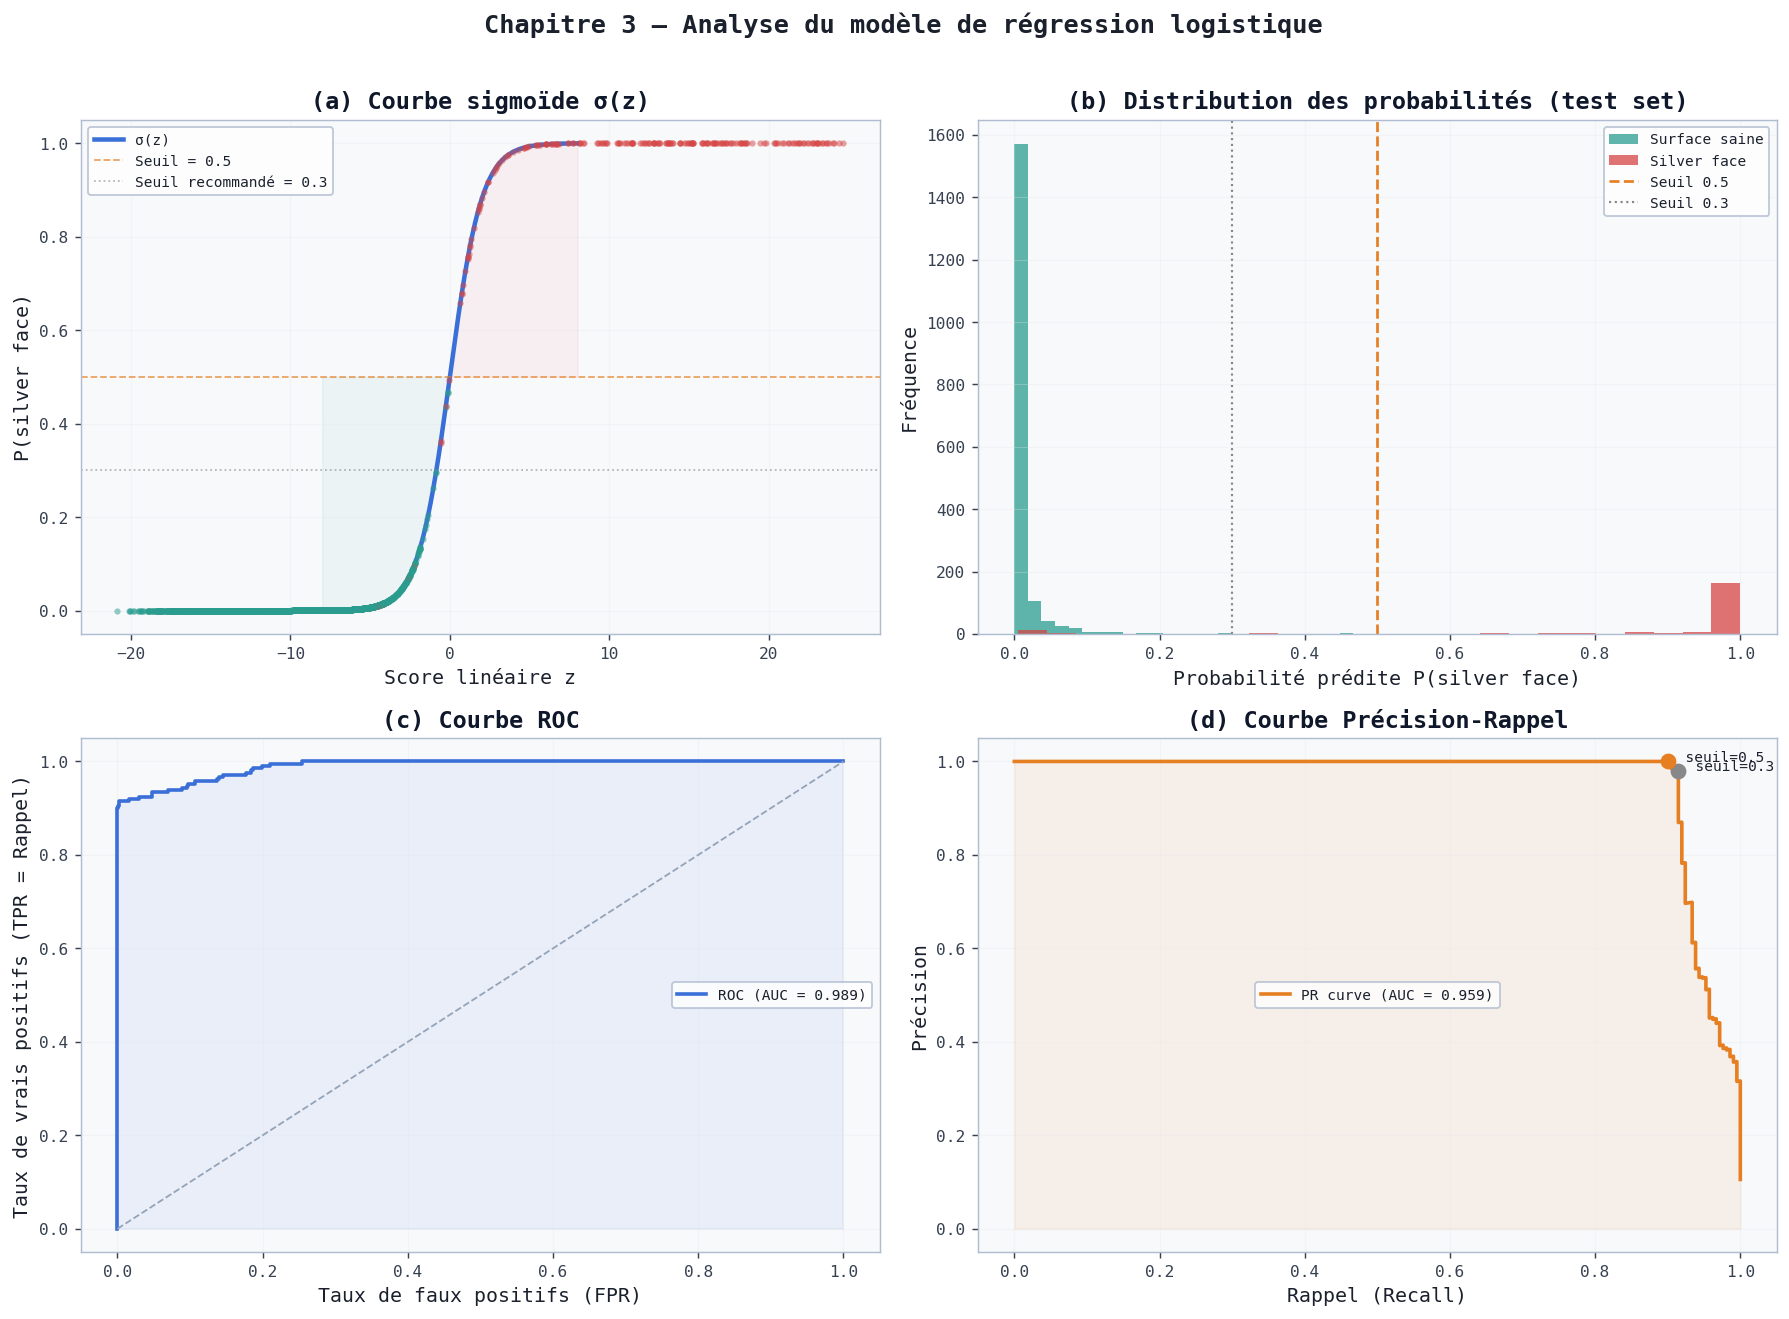
\includegraphics[width=\textwidth]{image/AI-SILVER-FACE/fig3_analysis.png}
    \caption{Analyse du modèle sur le jeu de test : (a)~sigmoïde $\sigma(z)$, (b)~distribution des probabilités prédites, (c)~courbe ROC (AUC~=~0,989), (d)~courbe Précision-Rappel (AUC~=~0,959).}
    \label{fig:analysis}
\end{figure}

Le panneau~(a) montre que chaque surface projetée sur la courbe sigmoïde selon son score linéaire $z$ se sépare nettement en deux nuages~; les rares points autour de $z \approx 0$ correspondent aux cas ambigus de la zone de chevauchement. Le panneau~(b) visualise le \textbf{recouvrement} entre les deux distributions~: plus les deux histogrammes sont séparés et étroits, plus le modèle est confiant.

La courbe ROC (panneau~c) représente le compromis entre le \textbf{taux de vrais positifs} (rappel, TPR) et le \textbf{taux de faux positifs} (FPR) pour tous les seuils $\tau$ possibles~:

\begin{equation}
    \text{TPR} = \frac{VP}{VP + FN}, \qquad \text{FPR} = \frac{FP}{FP + VN}
    \label{eq:tpr-fpr}
\end{equation}

La courbe PR (panneau~d) est particulièrement adaptée aux \textbf{jeux de données déséquilibrés} (ici 73~\% saines / 27~\% \textit{silver faces}). Elle représente le compromis entre~:

\begin{equation}
    \text{Précision} = \frac{VP}{VP + FP}, \qquad \text{Rappel} = \frac{VP}{VP + FN}
    \label{eq:precision-rappel}
\end{equation}

Dans un contexte de contrôle qualité, le \textbf{rappel} est prioritaire $\bullet$ manquer une \textit{silver face} (faux négatif) est plus coûteux qu'une fausse alarme. Un seuil abaissé à $\tau = 0{,}3$ augmente le rappel au prix d'une légère diminution de la précision.

\subsection{Frontière de décision}
\label{subsec:decision-boundary}

\begin{figure}[H]
    \centering
    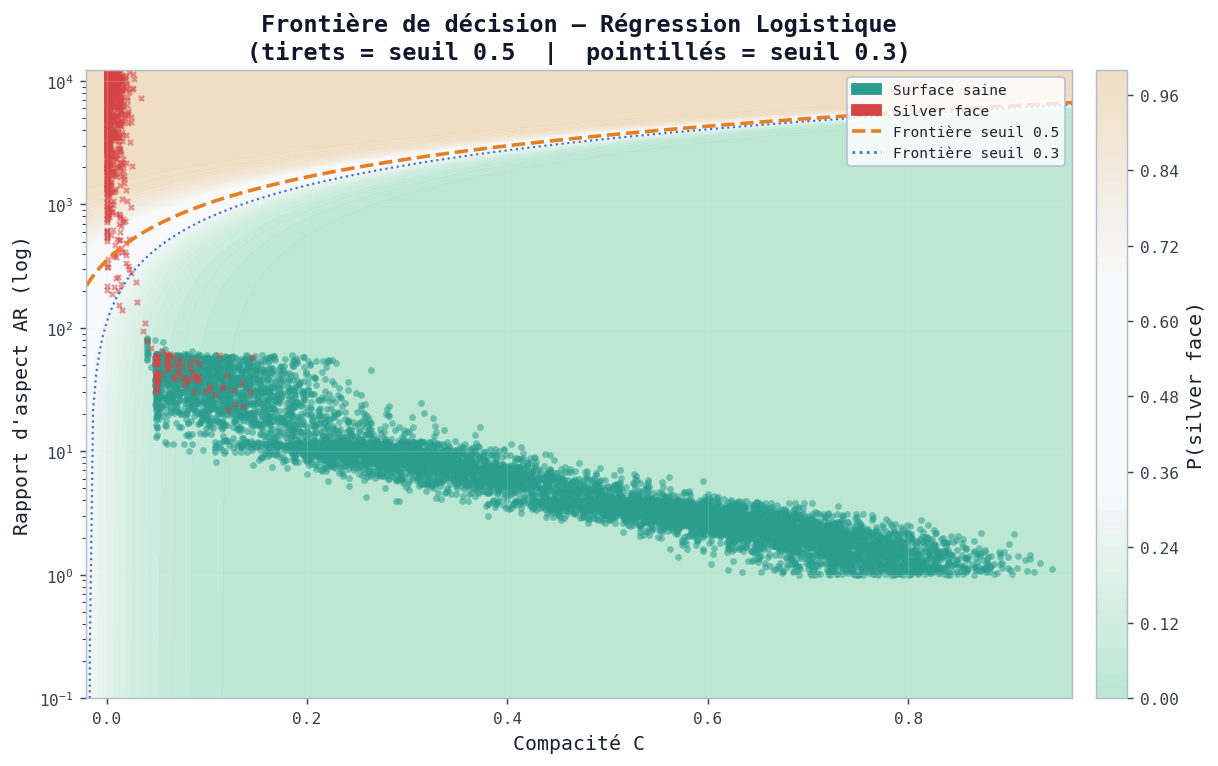
\includegraphics[width=0.9\textwidth]{image/AI-SILVER-FACE/fig4_decision_boundary.png}
    \caption{Frontière de décision dans le plan $C \times AR$ (tirets~: $\tau = 0{,}5$~; pointillés~: $\tau = 0{,}3$).}
    \label{fig:decision-boundary}
\end{figure}

Le seuil $\tau = 0.3$ est décalé vers la zone saine, ce qui permet de capturer davantage de \textit{silver faces} au prix d'un léger empiétement sur les surfaces saines ambiguës.

% ============================================================
\section{Métriques de classification}
\label{sec:metriques}
% ============================================================

Les matrices de confusion quantifient les performances du modèle pour les deux seuils de classification étudiés.

\subsection{Seuil standard \texorpdfstring{$\tau = 0.5$}{tau = 0.5}}
\label{subsec:confusion-05}

\begin{figure}[H]
    \centering
    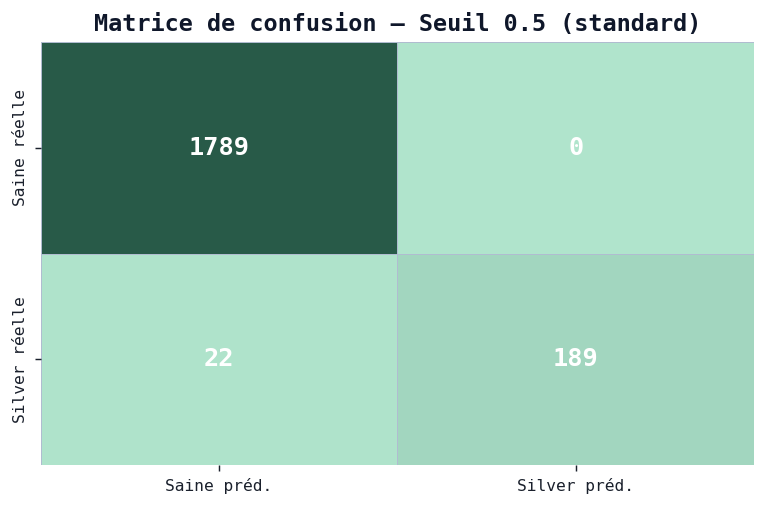
\includegraphics[width=0.65\textwidth]{image/AI-SILVER-FACE/fig5a_confusion_05.png}
    \caption{Matrice de confusion $\bullet$ seuil standard $\tau = 0{,}5$.}
    \label{fig:confusion-05}
\end{figure}

\subsection{Seuil recommandé \texorpdfstring{$\tau = 0.3$}{tau = 0.3}}
\label{subsec:confusion-03}

\begin{figure}[H]
    \centering
    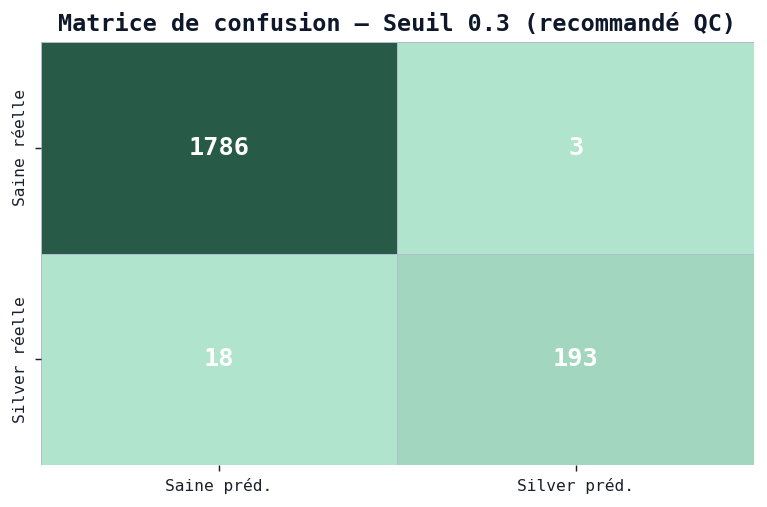
\includegraphics[width=0.65\textwidth]{image/AI-SILVER-FACE/fig5b_confusion_03.png}
    \caption{Matrice de confusion $\bullet$ seuil recommandé $\tau = 0{,}3$.}
    \label{fig:confusion-03}
\end{figure}

Les quatre cases de la matrice de confusion sont définies dans le \autoref{tab:confusion-matrix-def}.

\begin{table}[H]
    \centering
    \caption{Définition des cases de la matrice de confusion}
    \label{tab:confusion-matrix-def}
    \begin{tabularx}{\textwidth}{|X|>{\centering\arraybackslash}p{4cm}|>{\centering\arraybackslash}p{4.5cm}|}
        \hline
        \rowcolor{headerblue}
        \textcolor{white}{\textbf{}} &
        \textcolor{white}{\textbf{Prédit saine}} &
        \textcolor{white}{\textbf{Prédit \textit{silver face}}} \tabularnewline
        \hline
        \rowcolor{rowlight}
        \textbf{Réelle saine} & Vrais négatifs (VN) & Faux positifs (FP) \\
        \hline
        \rowcolor{rowwhite}
        \textbf{Réelle \textit{silver face}} & Faux négatifs (FN) & Vrais positifs (VP) \\
        \hline
    \end{tabularx}
\end{table}

Avec le seuil standard $\tau = 0.5$, le modèle ne classe \textit{silver face} que les cas très probables, réduisant les faux positifs mais augmentant le risque de faux négatifs. Avec $\tau = 0.3$, le modèle est plus sensible et détecte davantage de \textit{silver faces} réelles au prix de quelques fausses alarmes supplémentaires. Dans un pipeline de contrôle qualité automatisé, ce compromis est préférable.

% ============================================================
\section{Interprétabilité $\bullet$ Poids du modèle}
\label{sec:interpretabilite}
% ============================================================

\begin{figure}[H]
    \centering
    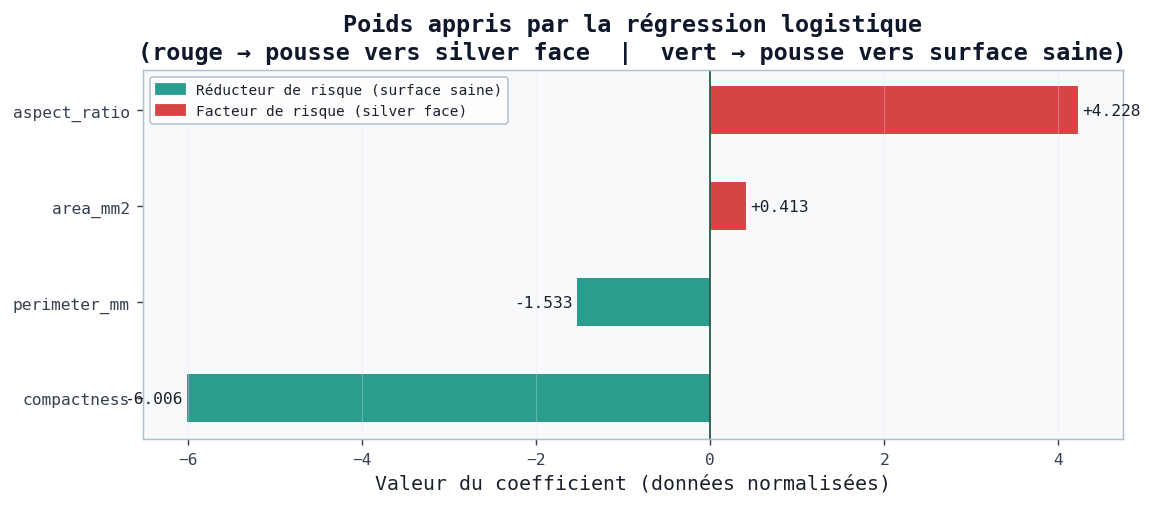
\includegraphics[width=0.85\textwidth]{image/AI-SILVER-FACE/fig6_weights.png}
    \caption{Coefficients appris par la régression logistique (rouge~: facteur de risque, vert~: réducteur de risque).}
    \label{fig:weights}
\end{figure}

Les poids $w_i$ indiquent la contribution de chaque caractéristique normalisée à la décision finale :

\begin{itemize}
    \item Le \textbf{rapport d'aspect} ($AR$, coefficient $+4.228$) est le facteur le plus influent en faveur d'une détection \textit{silver face} : plus $AR$ est élevé, plus la surface est suspecte.
    \item La \textbf{compacité} ($C$, coefficient $-6.006$) est le facteur protecteur dominant : une compacité élevée est une forte indication de surface saine.
    \item L'\textbf{aire} et le \textbf{périmètre} jouent un rôle secondaire, affinant la décision dans les cas ambigus.
\end{itemize}

% ============================================================
\section{Conclusion et recommandations}
\label{sec:innover-conclusion}
% ============================================================

Le modèle de régression logistique entraîné sur 1\,500 surfaces synthétiques démontre une capacité de discrimination robuste entre surfaces saines et \textit{silver faces}, avec une AUC-ROC de 0.989 et une AUC-PR de 0.959.

\textbf{Recommandations pour la mise en production :}

\begin{enumerate}
    \item \textbf{Seuil de classification} : utiliser $\tau = 0.3$ plutôt que le seuil standard 0.5, afin de maximiser la détection des \textit{silver faces} dans un contexte de contrôle qualité.
    \item \textbf{Indicateurs à surveiller} : la compacité $C$ et le rapport d'aspect $AR$ sont les deux signaux les plus discriminants. Une surface avec $C < 0.05$ et $AR > 100$ doit être systématiquement signalée.
    \item \textbf{Intégration CATIA} : le modèle peut être appelé depuis un script VBScript (\texttt{silver\_faces.vbs}) en extrayant les quatre caractéristiques géométriques via les APIs de mensuration CATIA~V5.
\end{enumerate}
